% StageSight technical report. Build from docs/paper:  latexmk -pdf stagesight.tex
\documentclass[conference,10pt,letterpaper]{IEEEtran}
\usepackage[T1]{fontenc}
\usepackage{newtxtext,newtxmath}
\usepackage{graphicx,booktabs,multirow,amsmath,xcolor,microtype}
\usepackage[skins]{tcolorbox}
\usepackage[hidelinks]{hyperref}
\graphicspath{{../figures/}}
\definecolor{cam}{HTML}{0C5DA5}
\newcommand{\cv}[1]{\texttt{\small cv.#1}}
\newtcolorbox{tracebox}[1]{enhanced, colback=cam!4, colframe=cam!70, boxrule=0.5pt, arc=1pt,
  left=3pt, right=3pt, top=2pt, bottom=2pt, fonttitle=\footnotesize\bfseries, title=#1, fontupper=\footnotesize}

\begin{document}
\title{StageSight: A River Camera That Checks Its Gauge\\
\large OpenCV~5 reads flood stage from USGS staff plates; a Claude agent on AWS decides which instrument to trust}
\author{\IEEEauthorblockN{Muhammad Waqar Saleem}
\IEEEauthorblockA{Department of Civil and Environmental Engineering, University of Missouri, Columbia, MO, USA\\
msx9t@missouri.edu \quad ORCID 0009-0004-4976-6979\\
OpenCV AI Competition 2026, powered by AWS}}
\maketitle

\begin{abstract}
A river gauge reports stage from a single pressure sensor; when that sensor drifts, freezes or
goes silent, often during the flood it exists for, the record gives no sign. Many USGS gauges
already carry a camera aimed at a staff plate, but its images are inspected by people, not
measured. StageSight turns that camera into an independent second instrument. Classical
OpenCV~5 operations and the OpenCV DNN text recognizer read the stage directly from the plate's
printed marks and numbers, \emph{without any gauge data}. On the 29~July~2026 flood at Hancock,
NY (USGS 01421500; NWS minor flood, 18.08~ft peak), the camera reads within 0.26~ft RMSE of the
USGS gauge (97\% within 0.5~ft, $n=30$), where a regression trained on normal flows misses by
6.3~ft. An event-gated agent (Claude Opus~4.6 on Amazon Bedrock) compares camera and gauge,
gathers evidence with tools, and queues sensor flags and flood alerts for human approval. In
replays with injected faults it catches all four gauge faults, two of them faster than a rule
baseline, and correctly blames the \emph{camera} in two camera-fault cases where the rules blame
the healthy gauge. The system runs live on AWS Lambda (Graviton), EventBridge, S3 and Bedrock,
and unchanged on a laptop CPU.
\end{abstract}

\section{Introduction}
Stage, the water level at a gauge, drives flood forecasts, warnings and discharge records.
Gauges fail in quiet ways: a sensor drifts with sediment, a pressure line freezes, telemetry
drops out. Hydrographers find these faults later, during record review; forecasters and
emergency managers may act on the bad value in real time.

The USGS operates cameras at many of its gauges and serves their images through the NIMS
API~\cite{nims}. Published camera methods measure stage from such images with deep
segmentation and photogrammetry~\cite{eltner2021,blanch2026} or learned
regression~\cite{vandaele2021,xu2025}, but they need surveyed control points, purpose-installed
cameras or training labels from the very gauge one would want to check. None uses the camera to
\emph{audit} the gauge.

\textbf{Contributions.}
\begin{enumerate}
\item A gauge-free reader for staff-plate cameras: the plate's own marks give a 1-D projective
pixel-to-feet map, the printed foot numbers (read with \cv{dnn.TextRecognitionModel}) give the
datum, and per-mark colour contrast gives the waterline. It reads a flood never seen in setup at
0.26~ft RMSE and returns an explicit status instead of a guess when it cannot see.
\item An event-gated agent that arbitrates between two instruments: code detects disagreement,
silence, blindness and flood levels; only then does Claude gather evidence (earlier frames, gauge
history, an upstream gauge) and act. A rule planner with the same tools is the baseline.
\item A safe operating design: agent memory, a safety net that always surfaces flood alerts,
a rule fallback, and a human approval queue; deployed serverless on AWS Graviton and evaluated
with injected gauge and camera faults on a real flood, including the agent's failures.
\end{enumerate}

\section{Related Work}
Eltner et al.~\cite{eltner2021} segment water with a CNN and intersect the waterline with a
photogrammetric 3-D model; Blanch et al.~\cite{blanch2026} run the same family for years at
dedicated stations, which requires surveyed ground control and installed cameras. Vandaele et
al.~\cite{vandaele2021} transfer-learn water segmentation on public river cameras but stop at
segmentation. Xu and Wang~\cite{xu2025} assess deep networks that regress gauge height from
webcam images; such models learn from the gauge record and are bounded by its range. StageSight
reads an absolute stage from the plate itself, so it needs neither survey nor training labels,
and it is designed to disagree with the gauge when the gauge is wrong.

\section{Data}
\textbf{Camera.} The NIMS ``Hancock Staff'' camera,
1080$\times$1920 frames, hourly, 21~Jul to 19~Oct~2026 (1,869 frames). The camera started on
14~Apr~2026; the 29~Jul event is its only flood. \textbf{Gauge.} USGS 01421500 gage height
(parameter 00065, 15-min), used \emph{only} for evaluation and by the agent as the instrument
under test. \textbf{Upstream.} USGS 01417500 at Harvard, NY (agent tool; 90-day
cross-correlation lag $\approx$3~h). \textbf{Flood levels.} NWS NWPS, HKCN6: action 14~ft,
minor flood 18~ft. All data are public.

\section{Reading the Plate with OpenCV 5}
\begin{figure*}[t]
\centering
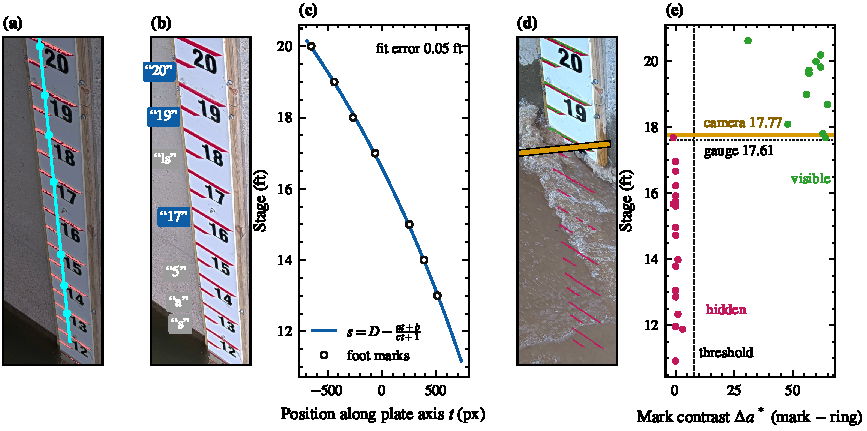
\includegraphics[width=\textwidth]{pipeline.pdf}
\caption{The reader on real frames. Setup on a dry frame, no gauge data: (a) HSV red mask and
robust plate axis (\cv{fitLine}, Huber) through the foot-mark centroids
(\cv{connectedComponentsWithStats}); (b) CRNN text recognition of the printed numbers; blue
reads vote for the datum, grey misreads cannot; (c) 1-D projective map from the foot marks.
Every frame, here at the flood peak: (d) marks still visible (green) and hidden under water
(magenta), waterline in yellow; (e) Lab $a^*$ contrast of each mark against its surround, on the
stage axis: visible marks sit far above the threshold, submerged marks at zero. Reading
17.77~ft; gauge 17.61~ft.}
\label{fig:pipeline}
\end{figure*}

\subsection{Setup, once per camera}
\textbf{Plate and marks.} Red pixels are found by an HSV threshold and a $3\times3$ opening;
\cv{fitLine} with a Huber loss gives the plate axis $\mathbf{d}$ through origin $\mathbf{o}$.
Each connected component is a mark; the long foot marks are kept (area $\geq 0.6\times$ the
median of the eight largest) and projected onto the axis, $t_i=(\mathbf{c}_i-\mathbf{o})^\top
\mathbf{d}$. Gaps of about twice the local spacing are indexed as a missing mark.

\textbf{Scale.} A pinhole camera maps points on a straight plate to the image line by a 1-D
homography, so plate units $u$ (ft below the top foot mark) follow
\begin{equation}
u(t)=\frac{a\,t+b}{c\,t+1},\qquad
\begin{bmatrix} t_i & 1 & -t_i u_i\end{bmatrix}
\begin{bmatrix} a\\ b\\ c\end{bmatrix}=u_i ,
\label{eq:homography}
\end{equation}
solved by linear least squares over the foot marks (fit error 0.05~ft, Fig.~\ref{fig:pipeline}c).
Three parameters, fixed by geometry, extrapolate along the plate in a way a free polynomial
does not.

\textbf{Datum.} The plate is rotated upright (\cv{warpAffine}); red is whitened and the black
digits under each foot mark are cropped. The OpenCV Zoo CRNN~\cite{shi2015crnn,zoo} runs through
\cv{dnn.TextRecognitionModel} (CTC greedy decoding). Each digit read $k$ at mark $i$ votes for
datum $D=k+u_i$. A dropped leading ``1'' is the usual misread, so only the longest reads may
vote. At Hancock the vote gives $D=20$~ft (6 of 7 votes). Stage is then $s=D-u$.

\subsection{Every frame}
\textbf{Quality gate.} Frames that are blurred (variance of the Laplacian $<40$), dark or
over-exposed are \texttt{rejected}.
\textbf{Registration.} The camera moves a few pixels between days. \cv{phaseCorrelate} on the
always-dry top of the plate (Hann-windowed) gives the shift $(\Delta x,\Delta y)$; above 80~px
the status is \texttt{camera\_moved}.
\textbf{Mark visibility.} For each of the $n=29$ marks, the median Lab $a^*$ inside the mark is
compared with a ring around it (\cv{dilate}, $15\times15$ minus $5\times5$):
\begin{equation}
v_j=\mathbf{1}\!\left[\operatorname{med}_{\text{mark }j}a^*-\operatorname{med}_{\text{ring }j}a^*\geq 8\right].
\end{equation}
The test is relative, so it holds in sun, shade and overcast; water and foam over a mark remove
its contrast (Fig.~\ref{fig:pipeline}e).
\textbf{Waterline.} With marks ordered top to bottom, the split
\begin{equation}
k^\star=\arg\min_k\;\textstyle\sum_{j<k}(1-v_j)+\sum_{j\geq k}v_j
\end{equation}
tolerates a few wrong marks (glare, a leaf). The waterline $t^\star$ is the midpoint of the gap
between mark $k^\star\!-\!1$ and mark $k^\star$, and $s=D-u(t^\star)$.
\textbf{Status.} $k^\star\geq n-1$ (only the lowest mark hidden, ambiguous at low water) gives
\texttt{below\_plate}; $k^\star=0$ gives \texttt{unreadable} (night infrared, fog, spray). The
reader never extrapolates below the plate.

\begin{figure*}[t]
\centering
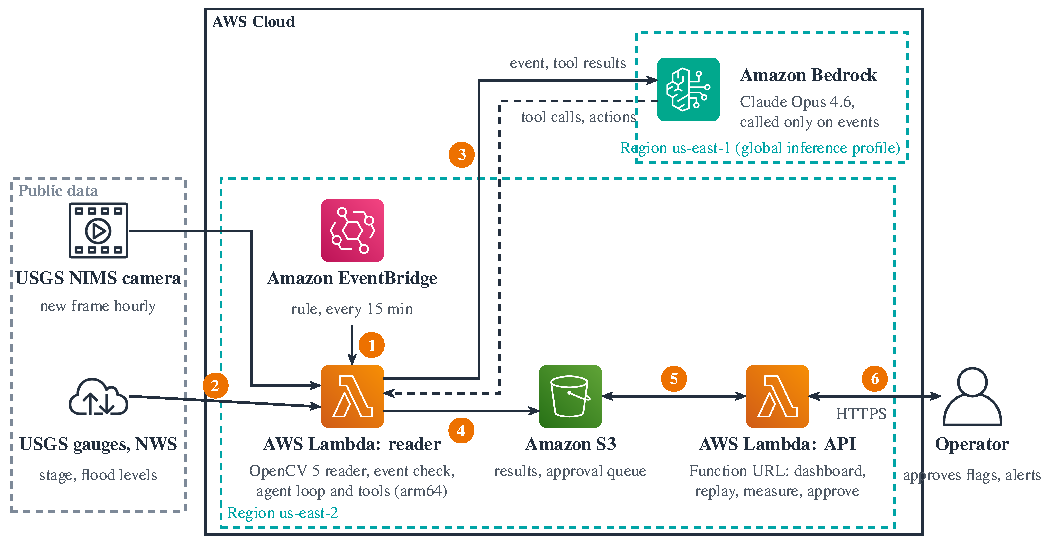
\includegraphics[width=0.92\textwidth]{architecture.pdf}
\caption{Deployment. \textcircled{\scriptsize 1} EventBridge starts the reader every 15~min;
\textcircled{\scriptsize 2} it fetches the newest frame and gauge values; \textcircled{\scriptsize 3}
on an event it calls Claude on Bedrock; \textcircled{\scriptsize 4} results and the approval queue
go to a private S3 bucket; \textcircled{\scriptsize 5}--\textcircled{\scriptsize 6} a second
Lambda serves the dashboard and takes approvals.}
\label{fig:arch}
\end{figure*}
\section{The Agent}
OpenCV runs on every frame; Claude is called only when code raises an event
(Table~\ref{tab:events}). The planner receives the event, the open issues and its own recent
actions (memory), and runs a manual tool loop with adaptive thinking through the Anthropic
Bedrock client. Evidence tools: \texttt{reread\_earlier\_frames} (re-runs the reader, including
mark counts), \texttt{get\_site\_gauge}, \texttt{get\_upstream\_gauge}. Final actions:
\texttt{flag\_sensor} and \texttt{draft\_alert} (both enter the approval queue),
\texttt{publish\_provisional\_stage}, \texttt{no\_action}. Two operator facts are in the
prompt: readings move in 0.5~ft steps, and upstream changes arrive about 3~h later.

\begin{table}[t]
\caption{Events that call the agent}
\label{tab:events}
\centering\footnotesize
\begin{tabular}{@{}ll@{}}
\toprule
Event & Trigger (code, every frame)\\
\midrule
\texttt{disagree} & camera and gauge differ $>0.5$~ft for 2 frames\\
\texttt{gauge\_silent} & camera reads, gauge has no recent value\\
\texttt{camera\_blind} & camera unreadable 3 frames, gauge $\geq$ action\\
\texttt{level\_rise} & camera or gauge reaches an NWS level\\
\bottomrule
\end{tabular}
\end{table}

\textbf{Safety design.} (i) \emph{Safety net}: a \texttt{level\_rise} always yields a flood
alert draft for the operator; if the agent doubted it, its doubt is written into the draft.
(ii) \emph{Fallback}: on throttling, API errors or a refusal the rule planner decides, and the
log says so. (iii) \emph{Human in the loop}: no flag or alert leaves the system without approval.

\section{System on AWS}

Both functions run on arm64 (Graviton) from one 78~MB zip that bundles the Linux arm64 wheels
of \texttt{opencv-python-headless}~5.0.0.93; it is built without Docker and deployed by an
idempotent script that creates the bucket, an IAM role, both functions, the schedule and a
Function URL (Fig.~\ref{fig:arch}). From CloudWatch, a scheduled tick (download, read, agent
check, write) takes a median of 6.3~s ($n=23$, peak memory 295~MB) and an API request 47~ms
($n=1{,}227$). At 96 ticks a day this is about 27,000~GB-s per month at the configured
1.5~GB. Claude is called only on events: none on a quiet day, two or three during the replayed
flood, about seven tool steps each.

\section{Experiments}
\subsection{Accuracy on a real flood}
Test frames are daylight frames in 21~Jul--1~Aug with the water on the plate ($n=30$). For the
baselines, 15 normal-flow frames (up to 11.97~ft) serve as training data; 27 of the 30 test
frames lie above that range.

\begin{table}[t]
\caption{Stage error on the 29 July 2026 flood ($n=30$)}
\label{tab:accuracy}
\centering\footnotesize
\setlength{\tabcolsep}{4pt}
\begin{tabular}{@{}lcccc@{}}
\toprule
Method & Gauge data & RMSE & Bias & $\leq$0.5 ft\\
\midrule
\textbf{StageSight} (ours) & none & \textbf{0.26} & $+0.07$ & \textbf{97\%}\\
Plate + gauge-fitted offset & training & 0.37 & $-0.27$ & 83\%\\
Linear pixel fit, normal flows & training & 6.31 & $-4.70$ & 23\%\\
\bottomrule
\multicolumn{5}{@{}l}{\scriptsize Errors in ft. StageSight MAE 0.21~ft, $R^2=0.99$.}
\end{tabular}
\end{table}

\begin{figure*}[t]
\centering
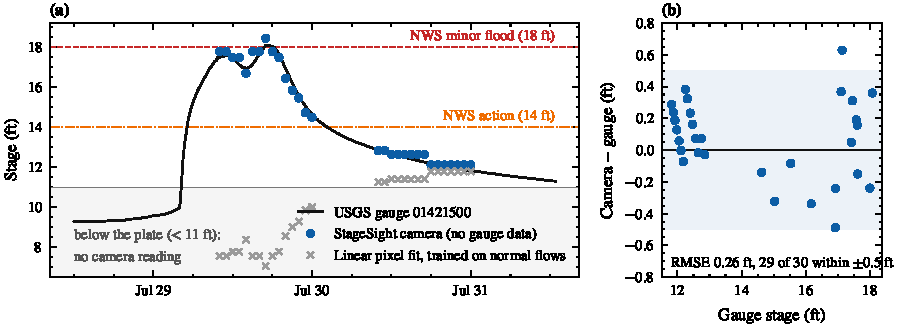
\includegraphics[width=\textwidth]{flood.pdf}
\caption{(a) The camera follows both flood peaks with no gauge data; a linear fit trained on
normal flows cannot reach flood stage. Below the plate (shaded) the reader reports
\texttt{below\_plate}. (b) Error against stage; the band is $\pm0.5$~ft, the plate's half-foot
mark spacing.}
\label{fig:flood}
\end{figure*}

Table~\ref{tab:accuracy} and Fig.~\ref{fig:flood}: StageSight is the only method without gauge
data and the most accurate. Marks are 0.5~ft apart, so a single reading is quantised to about
$\pm0.25$~ft; 0.26~ft RMSE is close to that floor. Fitting the offset to the gauge on normal
flows is \emph{worse} (0.37~ft): the lowest mark is often wet at low water, which biases the fit.
The learned baseline fails because it never saw a flood. Two flood frames are regression tests
in the repository (17.77 vs 17.61~ft; 12.63 vs 12.47~ft).

\textbf{Ablations.} A sub-mark edge search inside the bracket gave 0.275~ft against 0.257~ft for
the midpoint and was not adopted. Using the bracket between two marks as an uncertainty interval
covered the gauge in only 23--50\% of frames, so we do not claim intervals.

\subsection{Coverage}
\begin{figure*}[t]
\centering
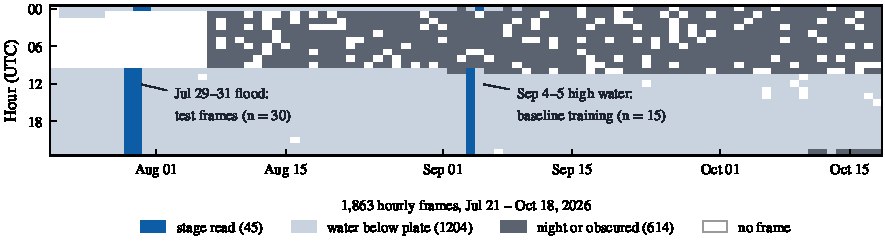
\includegraphics[width=\textwidth]{coverage.pdf}
\caption{Reader status for every hourly frame over 90 days (columns: days; rows: hour UTC).
The camera reads during the two high-water periods; otherwise the water is below the plate
(light) or it is night (dark).}
\label{fig:coverage}
\end{figure*}
Over 90 days the reader gave a number for 45 of 1,869 frames (2.4\%, Fig.~\ref{fig:coverage}).
The water was below the plate for 64\% of frames and 33\% were night infrared or fog. The plate
is a flood instrument: it reads when the river is high, which is when a gauge fault matters.

\begin{figure*}[t]
\centering
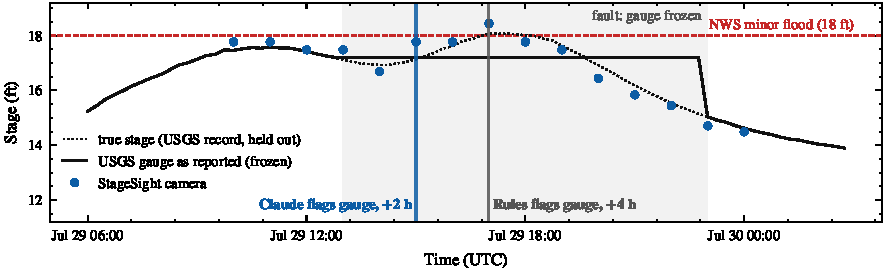
\includegraphics[width=\textwidth]{timeline.pdf}
\caption{Frozen-gauge replay. The reported gauge stays at 17.21~ft while the river rises to its
second peak and falls. Claude flags the gauge 2~h after the fault, citing the upstream gauge and
the camera; the rule baseline needs 4~h of consistent disagreement.}
\label{fig:timeline}
\end{figure*}
\subsection{Agent: injected faults on the real flood}
The replay feeds the 29~July flood frame by frame and injects four gauge faults and two camera
faults (Fig.~\ref{fig:faults}); the camera faults are synthetic overlays on real frames. The rule
planner uses the same tools with fixed thresholds.

\begin{table}[t]
\caption{Rules vs Claude on injected faults (single runs)}
\label{tab:agent}
\centering\footnotesize
\setlength{\tabcolsep}{3.5pt}
\begin{tabular}{@{}lll@{}}
\toprule
Fault & Rule baseline & Claude Opus 4.6\\
\midrule
none (flood only) & 0 false flags, 2 alerts & 0 false flags, 2 alerts\\
gauge offset +1 ft & flagged, 1 h & flagged, 1 h\\
gauge silent 8 h & camera published, 1 h & camera published, 1 h\\
gauge frozen 10 h & flagged, 4 h & \textbf{flagged, 2 h}\\
gauge drift to +1.5 ft & flagged, 8 h & flagged, 7 h\\
debris over plate & \textcolor{red!70!black}{blamed healthy gauge} & \textbf{blamed camera}\\
spray on lens & \textcolor{red!70!black}{blamed healthy gauge} & \textbf{blamed camera}\\
\bottomrule
\end{tabular}
\end{table}

\begin{figure}[t]
\centering
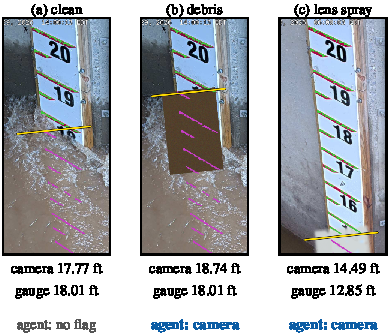
\includegraphics[width=\columnwidth]{faults.pdf}
\caption{Simulated camera faults on real frames, with the reader's output. (b) Debris hides
the marks from 16.6 to 18.8~ft, (c) spray removes their colour; the reader reads too high and
the gauge is right.}
\label{fig:faults}
\end{figure}



Both planners catch every gauge fault (Table~\ref{tab:agent}); Claude
flags the frozen gauge in half the time (Fig.~\ref{fig:timeline}). The difference is in the
camera faults: fixed thresholds see a persistent disagreement and blame the gauge, then publish
the bad camera stage. Claude checks the evidence and blames the camera (Fig.~\ref{fig:trace}).



In 90 days of normal operation (1,863 replayed ticks, rule planner) there were no false sensor
flags and two alerts, both at the real flood.

\begin{figure}[t]
\begin{tracebox}{{Claude, debris case, 19:00 UTC (verbatim excerpt)}}
\textbf{Tools:} \texttt{reread\_earlier\_frames(n=4)}, \texttt{get\_site\_gauge(12 h)},
\texttt{get\_upstream\_gauge(12 h)}.\\
\textbf{flag\_sensor(camera):} ``Camera reads 18.74 ft vs gauge 17.63 ft (+1.11 ft). Visible
marks fell from 11 to 7 even as the gauge recedes smoothly from its 18.06 ft peak. Upstream
gauge confirms falling trend with appropriate 3-hour lag.''
\end{tracebox}
\caption{An agent decision in the debris case: the evidence Claude gathered and the flag it queued for approval.}
\label{fig:trace}
\end{figure}

\subsection{Development history of the agent}
We report all three Claude runs. \emph{Run 1} missed the drift (it blamed the camera); the two
operator facts above were added. \emph{Run 2} caught every fault but, in the frozen-gauge case,
forgot its own gauge flag and drafted \emph{no flood alert during a real flood}. The fix was in
the system, not the prompt: memory of open issues and the safety net. \emph{Run 3}
(Table~\ref{tab:agent}): the safety net fired once, again in the frozen-gauge case: Claude
reasoned from the 3~h lag that the river should be falling, but this flood peaked about 7~h
after the upstream peak. We did not re-tune the lag to this flood. The evaluation has clear
limits: one flood, one run per scenario, and prompt facts added after seeing run~1.

\section{Limitations and Failure Cases}
\textbf{Night}: infrared frames show the plate but not the red marks (\texttt{unreadable}).
\textbf{Low water}: below about 11~ft the plate is dry and the camera cannot check the gauge.
\textbf{Plate designs}: other NIMS plates (Owasco, Moravia, Chenango, NY) use black marks or
0.1~ft text, or stand on dry bank; they are not supported yet. \textbf{No plate}: a
self-calibrated research mode learns a per-pixel flood-stage map from the archive (0.29~ft MAE in
range on the Hancock wall) but does not extrapolate to floods; on far-bank bridge cameras
(Hermann, MO; De Soto, KS; 2--3~px per ft) it reaches only 3.4 and 2.3~ft RMSE in range.
\textbf{Model}: Claude Opus~4.6 is the most capable Claude model enabled on the new AWS account;
the model is one setting.

\section{Responsible Operation}
StageSight is a decision aid, not an official warning system. Nothing is sent without a
person's approval, and camera stages are labelled provisional. It uses public data only and no
personal data. The bucket is private; the Lambda role can write only that bucket and invoke
Bedrock models. The public Function URL serves read-only data; the approve endpoint is open in
this demonstration and would sit behind authentication in operation. Every agent decision,
tool call and reason is logged and shown on the dashboard.

\section{Conclusion}
A camera that already watches a staff plate can measure stage by geometry and OCR alone,
through a flood no learned model saw, and that independent reading lets an agent tell which
instrument is wrong. Next: read night infrared frames from the printed numbers, support more
plate designs across the NIMS network, and repeat the agent runs to report catch rates.

\textbf{Reproducibility.} Code, results and figures are at \url{https://github.com/Waqar-msx9t/stagesight} (Python~3.12,
OpenCV 5.0.0.93, NumPy 2.5.4, Anthropic SDK 1.15.0). The plate tests run offline; three scripts
(\emph{plate\_test}, \emph{replay\_agent}, \emph{make\_figures}) reproduce every number and figure.

\begin{thebibliography}{9}
\bibitem{nims} U.S. Geological Survey, ``National Imagery Management System (NIMS) API,'' \url{https://api.waterdata.usgs.gov/nims/v0}, accessed Oct.~2026.
\bibitem{eltner2021} A. Eltner, P. O. Bressan, T. Akiyama, W. N. Gon\c{c}alves, and J. Marcato Junior, ``Using deep learning for automatic water stage measurements,'' \emph{Water Resources Research}, 2021, doi:10.1029/2020WR027608.
\bibitem{blanch2026} X. Blanch, J. Grundmann, R. Hedel, and A. Eltner, ``AI image-based method for a robust automatic real-time water level monitoring: a long-term application case,'' \emph{Hydrology and Earth System Sciences}, vol.~30, p.~797, 2026, doi:10.5194/hess-30-797-2026.
\bibitem{vandaele2021} R. Vandaele, S. L. Dance, and V. Ojha, ``Deep learning for automated river-level monitoring through river-camera images: an approach based on water segmentation and transfer learning,'' \emph{Hydrology and Earth System Sciences}, vol.~25, p.~4435, 2021, doi:10.5194/hess-25-4435-2021.
\bibitem{xu2025} R. Xu and B. Wang, ``Assessing deep learning techniques for remote gauging and water quality monitoring using webcam images,'' \emph{Hydrology}, vol.~12, no.~4, p.~65, 2025, doi:10.3390/hydrology12040065.
\bibitem{shi2015crnn} B. Shi, X. Bai, and C. Yao, ``An end-to-end trainable neural network for image-based sequence recognition and its application to scene text recognition,'' arXiv:1507.05717, 2015.
\bibitem{zoo} OpenCV, ``OpenCV Zoo: text recognition CRNN (text\_recognition\_CRNN\_EN\_2021sep),'' \url{https://github.com/opencv/opencv_zoo}.
\end{thebibliography}
\end{document}
